% vim:spelllang=ru,en
\documentclass[a4paper,12pt,notitlepage,headsepline,pdftex]{scrartcl}

\usepackage{cmap} % чтобы работал поиск по PDF
\usepackage[T2A]{fontenc}
\usepackage[utf8]{inputenc}
\usepackage[english,russian]{babel}
\usepackage{concrete}
\usepackage{cite}
\usepackage{url}

\usepackage{textcase}
\usepackage[pdftex]{graphicx}

\usepackage{lscape}

\pdfcompresslevel=9 % сжимать PDF
\usepackage{pdflscape} % для возможности альбомного размещения некоторых страниц
\usepackage[pdftex]{hyperref}
% настройка ссылок в оглавлении для pdf формата
\hypersetup{unicode=true,
            pdftitle={6ой этап выполнения проекта по ПО ЭВМ},
            pdfauthor={Погода Михаил},
            pdfcreator={pdflatex},
            pdfsubject={},
            pdfborder    = {0 0 0},
            bookmarksopen,
            bookmarksnumbered,
            bookmarksopenlevel = 2,
            pdfkeywords={},
            colorlinks=true, % установка цвета ссылок в оглавлении
            citecolor=black,
            filecolor=black,
            linkcolor=black,
            urlcolor=blue}

\usepackage{amsmath}
\usepackage{amssymb}
\usepackage{moreverb}
\usepackage{indentfirst}
\usepackage{misccorr}

\usepackage{xtab}
\usepackage{nccfoots}

\begin{document}
\begin{titlepage}
  \begin{center}
    \large
    \MakeUppercase{Министерство образования и науки,}

    \MakeUppercase{молодёжи и спорта Украины}

    \mbox{\MakeUppercase{Национальный технический университет Украины}}

    \MakeUppercase{,,Киевский политехнический институт''}

    \addvspace{6pt}

    \normalsize
    Кафедра прикладной математики

    \vfill

    \textbf{Етап №6}

    выполнения курсового проекта

    по дисциплине ,,Программное обеспечение ЭВМ''

    \emph{Разработка алгоритмов}
  \end{center}

  \vfill

  \noindent
  Выполнил\\
  студент группы КМ-92\\
  Погода~М.\,В.\\
  \vfill

  \begin{center}
    КИЕВ

    2012
  \end{center}
\end{titlepage}

\begin{figure}[h]
  \begin{center}
    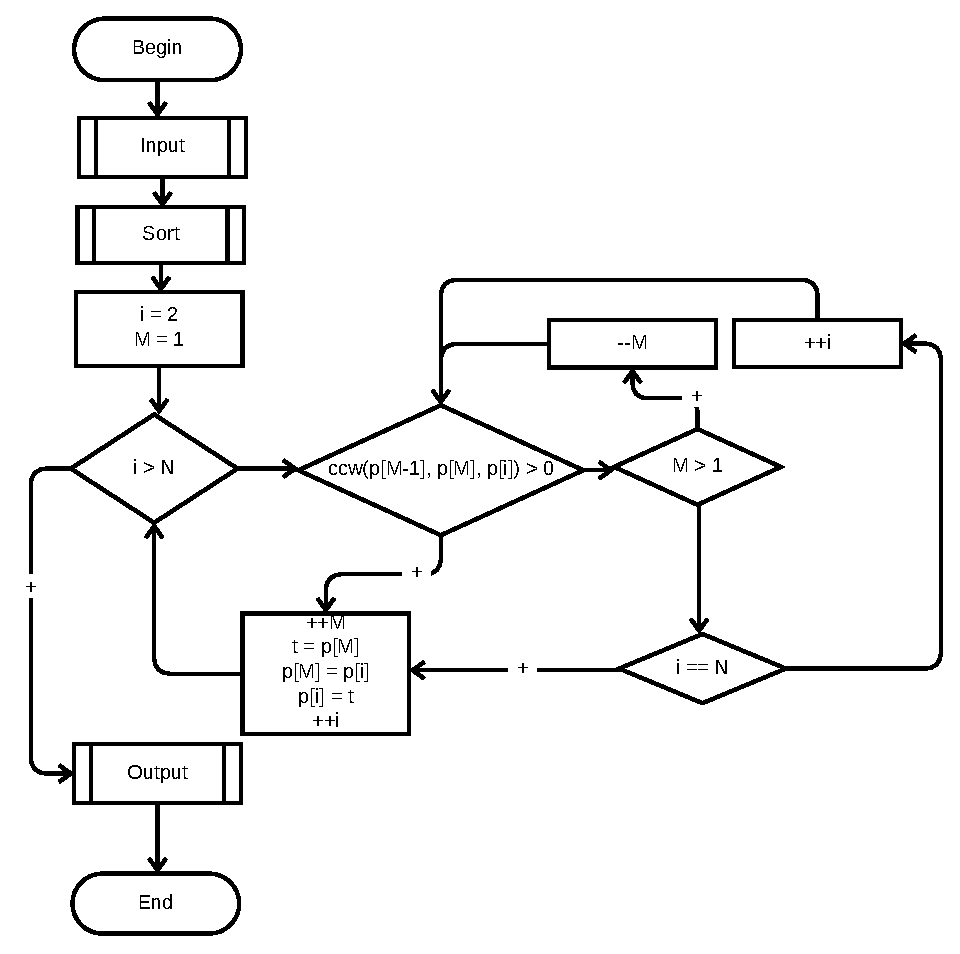
\includegraphics{algo.eps}
  \end{center}
  \caption{Блок"=схема работы алгоритма}
  \label{fig:algo}
\end{figure}

\begin{figure}[h]
  \begin{center}
    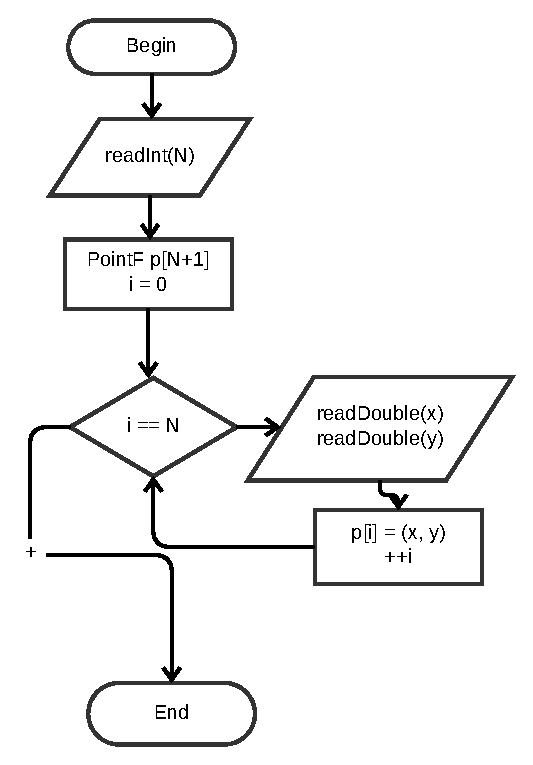
\includegraphics{input.eps}
  \end{center}
  \caption{Блок"=схема ввода данных}
  \label{fig:input}
\end{figure}

\begin{figure}[h]
  \begin{center}
    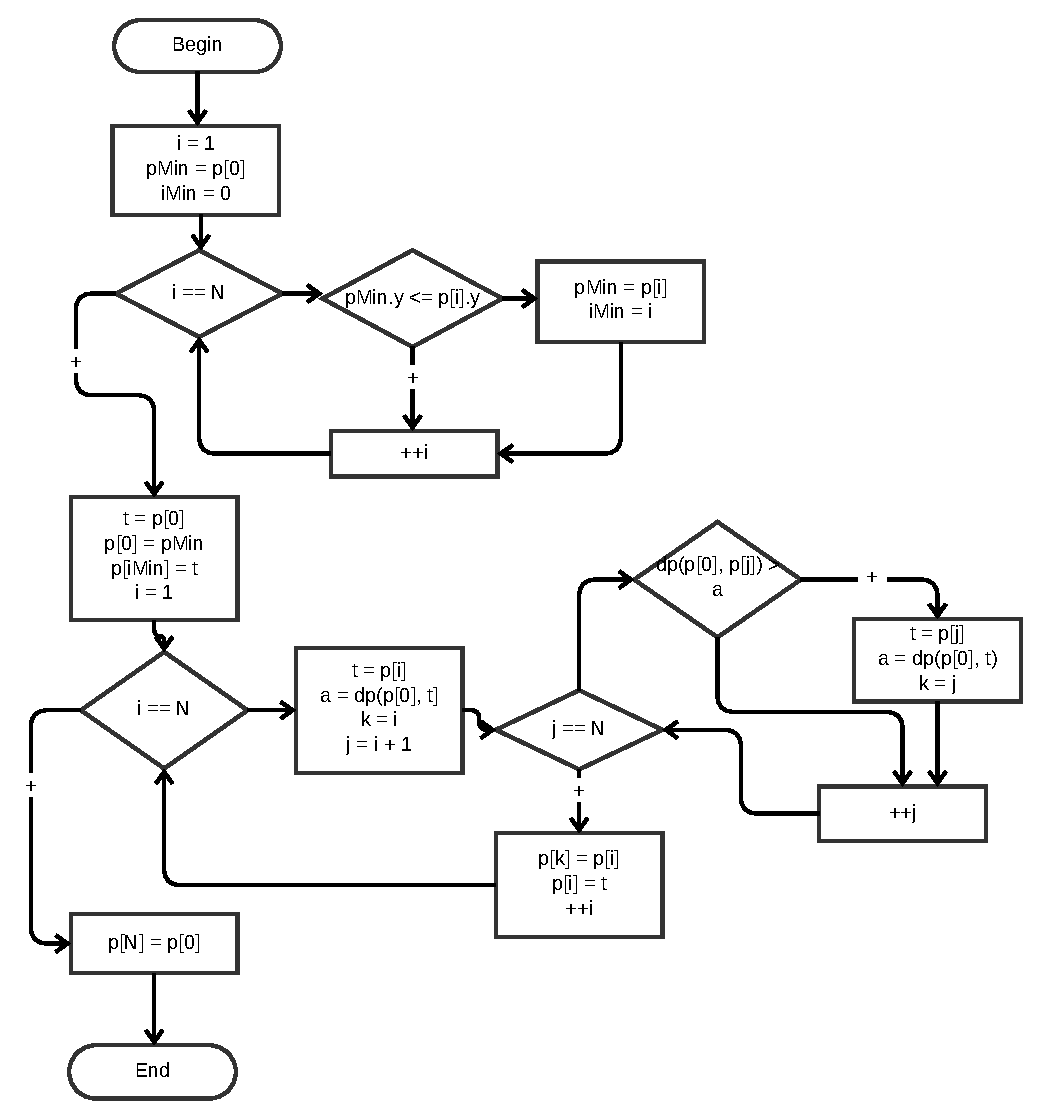
\includegraphics{sort.eps}
  \end{center}
  \caption{Блок"=схема подготовки массива к работе}
  \label{fig:sort}
\end{figure}

\begin{figure}[h]
  \begin{center}
    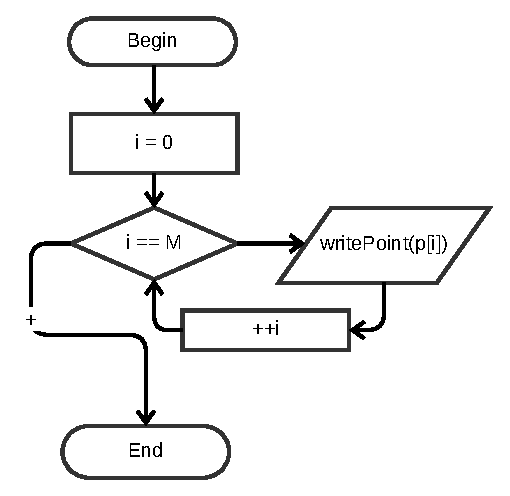
\includegraphics{output.eps}
  \end{center}
  \caption{Блок"=схема вывода результата}
  \label{fig:output}
\end{figure}

\end{document}
